\chapter{Design and Development of MC2101}
The present Chapter is entirely dedicated to MC2101 microcontroller. The first Section explains the hardware-level architecture of MC2101, from the bus infrastructure to the various peripherals, and all the related design and development choices. The software part is described in the second Section, dedicated precisely to describe all the implemented system's libraries provided to support the programmer job with a proper set of low-level C functions, useful to program all peripherals without the need of accessing their registers ``by hand''. A third Section is dedicated to the testing part, in particular to the testing methodology followed to assess the functional correctness of the various designed hardware components, and their interconnection. The same Section is also dedicated to describe how does the serial communication between FPGA and a PC have been implemented, with the purpose of providing a way to allow the interaction between a personal computer and the synthesized MC2101, through a command-line terminal.

\section{MC2101 architecture}
MC2101 microcontroller has been designed with the purpose of being used as a synthesizable and extensible platform for integration and assessment of security solution for IoT implemented inside the AFTAB processor. At the current state, the microcontroller is composed of a minimal set of peripherals properly selected for providing all necessary input/output functionalities useful for interacting with the external world, once synthesized on a FPGA.

%\begin{figure}[h!]
\begin{figure}[h]
\vspace{0.5cm}
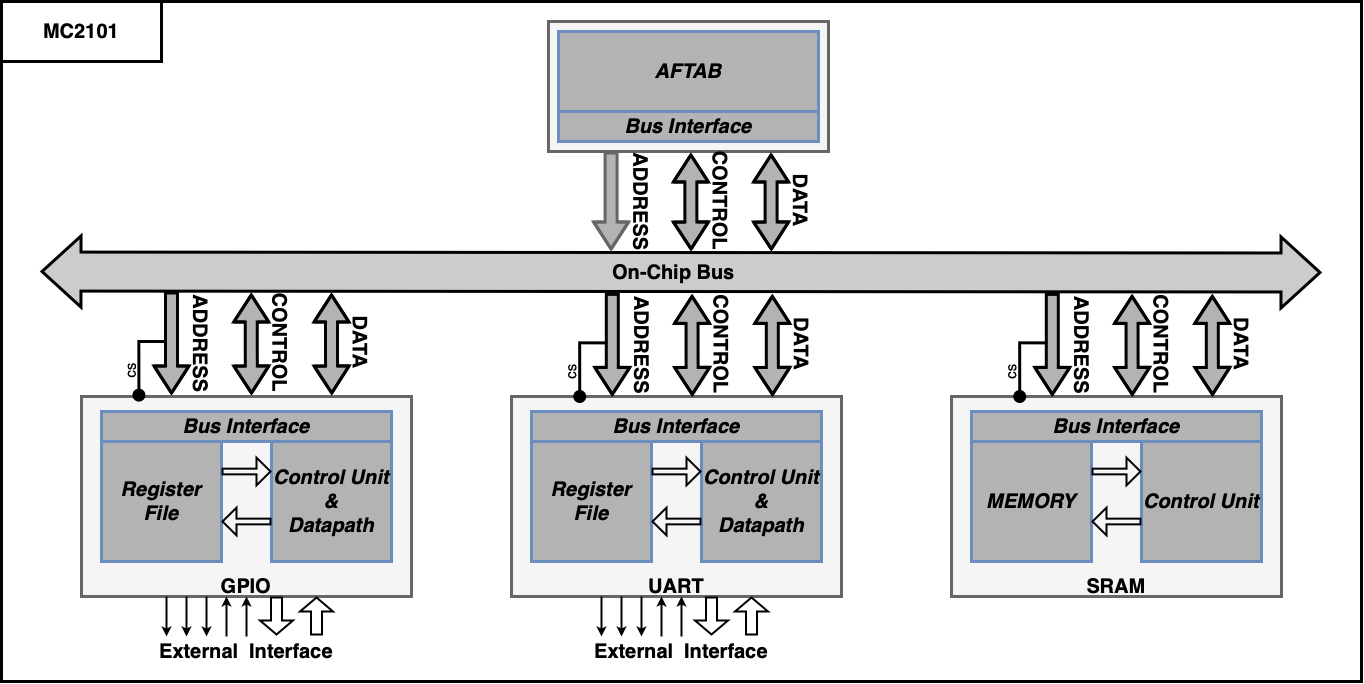
\includegraphics[width=\textwidth]{./images/MC2101}
\caption{MC2101 microcontroller.}
\label{fig:mc2101} % \ref{fig:mc2101}
\end{figure}

The Figure \ref{fig:mc2101}  shows the design overview of the microcontroller. The architecture includes a single bus, which provides the system with the proper hardware infrastructure necessary to interconnect the AFTAB processor with all peripherals and the main memory. The processor plays the role of the master: it is the only component able to initiate transactions on the bus, which can be composed of single or multi-cycles read/write operations. Peripherals and main memory are accessed by AFTAB using the memory-mapped mode: this means that the entire address space includes both peripherals and main memory. Therefore, the processor uses the same load/store instruction for accessing all components attached to the bus.

The communication between the processor and any peripheral happen only through the peripheral's register file, which can contain three different type of registers, with different read/write policy:

\begin{itemize}
\item \textbf{Control Registers}: used to configure the peripheral functionalities. They are written by the processor and read by the peripheral;
\item \textbf{Status Registers}: used to report the current state of the peripheral. Written by the peripheral and read by the processor;
\item \textbf{Data Registers}: used to exchange data. Both processor and peripheral can read and write on them.
\end{itemize}

The size and the number of registers depends on the functionalities implemented by the peripheral, which can be for instance a 32-bit peripheral, with 32-bit register file or a 8-bit peripheral with 8-bit registers. 

The bus implements three different types of interconnections:

\begin{itemize}
\item \textbf{Data Lines}: set of independent read and write data signals used to read and write data on peripherals registers and on the main memory;
\item \textbf{Control Lines}: used to provide signals for controlling read or write operations and for allowing peripherals and main memory to feedback the processor about the current state of the transaction;
\item \textbf{Address Lines \& Chip Select}: the most significant bits of the address lines pass through a decoder that drives all chip select signals: in this way, the peripheral is activated only when necessary.
\end{itemize}

Each component attached to the bus must include the Bus Interface, which is a sort of wrapper to be placed around each component in such a way to bridge signals coming from the bus to the internal hardware (FSM + Datapath) of the peripheral and vice versa. Peripherals can implement an additional External Interface, which is used to handle the communication to the external world. In particular, the conversion of incoming external asynchronous digital signals into the synchronous domain of the microcontroller.

In the following Subsection, some more details of the microcontroller design are reported, in order to present what are the functionalities supported by the system and the relative design choices made.

\subsection{Bus Infrastructure}
In the microcontroller development, the bus infrastructure was the first item to be addressed because of its vital role in interconnecting the whole system. In literature, there exist a lot of bus architectures which, over the years, have evolved to become an open-standard in SoCs design. In particular, the the most used open-source architecture is the ARM AMBA bus \cite{ambaAHB} \cite{ambaAPB}, that, thanks to its modular design engineered to support high-performance and low power on-chip communications, is today a standard \emph{de facto}, used in most of the SoCs present on the market. The problem with such solutions is that they implements sophisticated features, designed to be used in full-featured high-performance microcontrollers much more complex than our embedded system. In particular, the absence of a pipeline in the our processor prevents the usage of AMBA solutions, that are in fact designed to pipeline all the communications in order to increase the throughput.

The idea was to take inspiration from a standard architecture (AMBA and Avalon, for instance) to build a simpler infrastructure. In particular, the designed architecture preserves a minimal subset of AMBA specifications to build a simpler infrastructure, suitable for our needs, that remains modular and upgradable at the same time.

\begin{figure}[h]
\vspace{0.5cm}
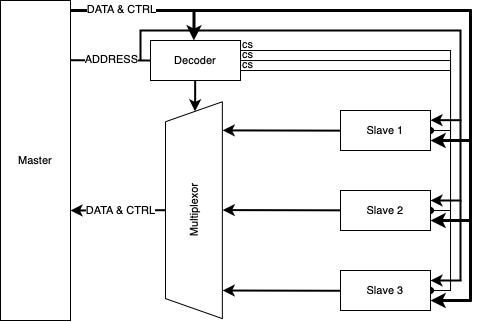
\includegraphics[scale=0.8]{./images/BUS}
\caption{MC2101 Bus Block Diagram.}
\label{fig:bus} % \ref{fig:bus}
\end{figure}

Figure \ref{fig:bus} shows the block diagram of the bus system. It is an infrastructure that supports a single master with multiple slaves, thus no arbitration mechanism has been implemented. The bus interconnection logic consists of a single centralised address decoder and a slave-to-master multiplexor. The decoder monitors the address lines driven by the master so that the appropriate slave is selected during each transaction. It also provides control to the multiplexor, which is in charge of routing the corresponding slave output back to the master.

%\begin{figure}[h!]
\begin{figure}[h]
\vspace{0.5cm}
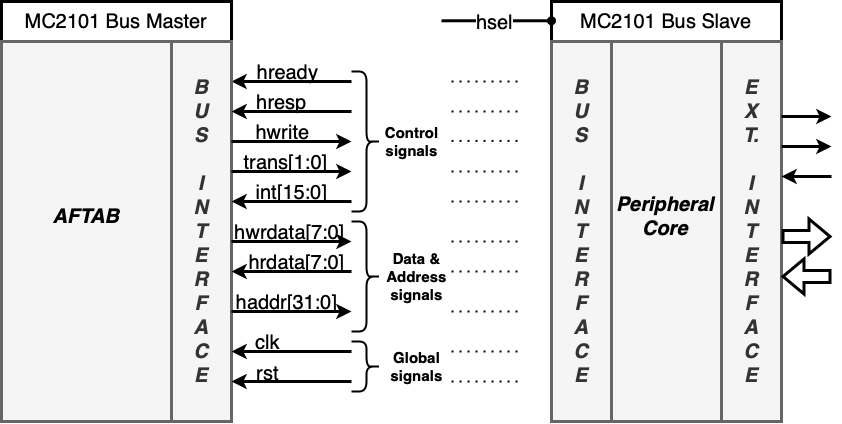
\includegraphics[scale=0.5]{./images/MasterSlave}
\caption{Master \& Slave Interfaces.}
\label{fig:masterslave} % \ref{fig:masterslave}
\end{figure}

The bus master interface, on the left of Figure \ref{fig:masterslave}, provides address and control information to initiate read and write operations.
The slave, whose interface is shown on the right of Figure \ref{fig:masterslave}, responds to transfers initiated by the master, by using a \texttt{hsel} (chip select) signal from the decoder to control when to respond a request. When selected, the slave will start monitoring the bus lines in order to respond to commands from the master. Therefore, all the slaves will stay into an idle state until they are individually waken up by a signal.\vspace{5mm} \newline 
Each slave is also able to feedback the master about:
\begin{itemize}
\item the success
\item the failure
\item or the waiting of the data transfer
\end{itemize}
by using the \texttt{hresp} and \texttt{hready} dedicated lines. In this way, a slave is able to extend the data phase when extra time is needed, but also to inform the rest of the system that some bad operations are happening in the bus.
\begin{table}
\centering
\begin{tabular}{| l | l | p{7cm} |}
    \hline
    \textbf{Name} & \textbf{Type} & \textbf{Description}\\ \hline
    \texttt{hready} & Control & When driven LOW, the transfer is extended.  \\ \hline
    \texttt{hresp} & Control & When HIGH, indicates that the transfer status is on error.  \\ \hline
    \texttt{hwrite} & Control & Indicates the transfer direction. When HIGH the signal implies a write transfer, on the contrary when LOW a read transfer.\\ \hline
    \texttt{htrans[1:0]} & Control & Shows the current state of the bus.\\ \hline
    \texttt{int[15:0]} & Control & Independent interrupt lines, can be driven by peripherals to issue a IRQs. \\ \hline
    \texttt{hwrdata[7:0]} & Data & 8-bit data lines from the master to the slaves. \\ \hline
    \texttt{hrdata[7:0]} & Data & 8-bit data lines from the slave to the master.  \\ \hline
    \texttt{haddr[31:0]} & Address & Address space is on 32-bit, thus also the address line. \\ \hline
    \texttt{clk} & Global & global clock signal \\ \hline
    \texttt{rst} & Global & global reset signal \\ \hline
    \hline
\end{tabular}
\caption{Bus Signals.}
\label{tab:bussig} % \ref{tab:bussig}
\end{table}
The full list of signals is described in Table \ref{tab:bussig}.

In the following Subsections, the main features implemented in the GPIO and UART peripherals are presented. Together, they provide a set of minimal functionalities for interacting with the microcontroller from the external world.

\subsection{GPIO Peripheral}
The GPIO (General Purpose Input Output) is a peripheral module present in all embedded processors. It is used to manage sets of SoC's incoming and outgoing digital signals, by driving and checking the logic state of physical pins. GPIOs can be used in a diverse variety of applications, limited only by the electrical and timing specifications of the peripheral's interface, and the ability of software to interact with it in a sufficiently timely manner. In most of the cases, GPIOs are used to switch LEDs, interface the microcontroller to buttons, user-selectable switches or electronic switches (relays). In other cases, there is also the possibility to use GPIO as a bit banging communication interface, where software is used as substitute for dedicated hardware in order to implement a specific communication protocol, e.g., a software-based SPI bus with 4 GPIO pins.

\begin{figure}[h]
\vspace{0.5cm}
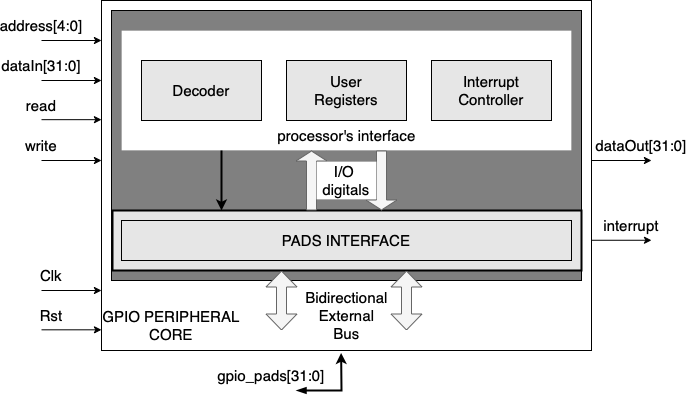
\includegraphics[width=\textwidth]{./images/GPIO}
\caption{MC2101 GPIO Peripheral Core.}
\label{fig:gpio} % \ref{fig:gpio}
\end{figure}

In Figure \ref{fig:gpio}, the core of the peripheral is showed, together with its relative set of signals coming from the Bus Interface and from the External Interface.
The GPIO is designed as a 32-bit peripheral, and so it provides a 32-bit processor's interface with 32-bit wide user registers and data bus (\texttt{dataIn} and \texttt{dataOut}). The conflict between MC2101's data bus, that is on 8-bit (see \texttt{hwrdata} and \texttt{hrdata} in Table \ref{tab:bussig}), and the peripheral's data bus are solved by the Bus Interface, which provides a bridge for the communications between the two domains. The External Interface (in Figure \ref{fig:gpio} as \emph{Pads Interface}) works as an intermediate between the bidirectional bus connected to physical pins and the peripheral's core. In particular, through the Pads Interface, the asynchronous bidirectional external lines (\texttt{gpio\_pads}) are separated into independent input and output lines, synchronised with the global clock.

The 5-bit \texttt{address} signal selects which user register is being access by the by the processor. As explained before, read and write operations on peripherals are enabled by a proper chip select signal. When the chip select condition is met, the Bus Interface rises one of the two strobe signals, \texttt{read} and \texttt{write}, for accessing the user registers. The GPIO provides also an \texttt{interrupt} line to the processor. This line will rise as soon as an interrupt condition occurs on any of the 32 pad lines. When this happen, the processor will have to execute appropriate read or write operations to deassert the interrupt. The peripheral, programmed through the user registers, is able to support the following functionalities:

\begin{itemize}
\item Control the input/output direction of each GPIO pads;
\item Enable interrupts for each input bits and configure the triggering behaviour on logic levels or rising/falling edges;
\item Drive and control external pins.
\end{itemize}

\begin{table}
\centering
\begin{tabular}{| p{2cm} | p{2cm} | p{2cm} | p{7cm} |}
    \hline
    \textbf{Name} & \textbf{Address} & \textbf{Access} & \textbf{Description}\\ \hline
    \texttt{PADDIR} & \texttt{0x1A100000} & R/W & Control the direction of each of the GPIO pads. A value of 1 means the pin is configured as output.  \\ \hline
    \texttt{PADIN} & \texttt{0x1A100004} & R & Saves the input values coming from input pins.\\ \hline
    \texttt{PADOUT} & \texttt{0x1A100008} & R/W & Drives the output lines with its content.\\ \hline
    \texttt{PADINTEN} & \texttt{0x1A10000C} & R/W & Interrupt enable bits for input lines.\\ \hline
    \texttt{INTTYPE} & \texttt{0x1A100010} & R/W & Two registers: \texttt{INTTYPE0}, \texttt{INTTYPE1} that are used to control the interrupt triggering behavior of each interrupt-enabled pin. \\ \hline
    \texttt{INTSTATUS} & \texttt{0x1A100018} & R & Contains interrupt status for each GPIO line. The interrupt line is high when a bit is set in this register and will be de-asserted when this register is read.\\ \hline
    \hline
\end{tabular}
\caption{GPIO User Registers.}
\label{tab:gpio} % \ref{tab:gpio}
\end{table}

From the programmer's point of view, the GPIO peripheral can be programmed through the set of registers in Table \ref{tab:gpio}. More details on the software are provided in the next Section, dedicated to the software part.

\subsection{UART Peripheral}
Communication protocols play very important role in organising communication between devices, which is a fundamental feature to be implemented, as it allows a way for interaction between different platforms. In fact, every embedded system includes at least one hardware peripheral dedicated for this role. Microcontrollers and computers mostly use UART as a form of device-to-device communication protocol, which only requires two wires to implement transmission and reception of data.

\begin{figure}[h]
\vspace{0.5cm}
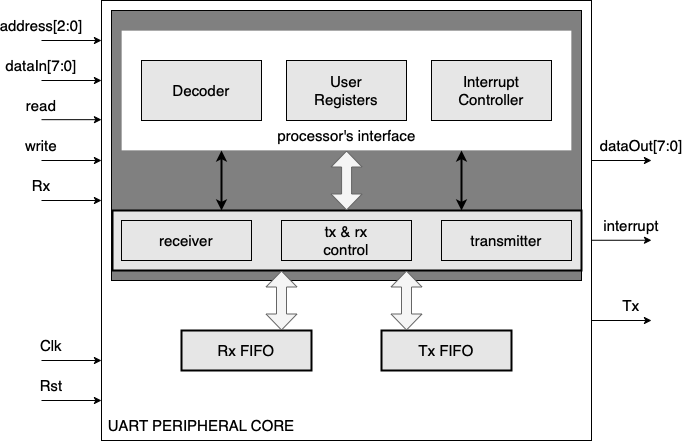
\includegraphics[scale=0.6]{./images/UART}
\caption{MC2101 UART Peripheral Core.}
\label{fig:uart} % \ref{fig:uart}
\end{figure}

The UART module designed for MC2101, whose block diagram is shown in Figure \ref{fig:uart}, provides a transmitter-receiver pair, configurable for different speeds, data widths, parity codifications and information status for several error conditions. The implementation provides a subset of the standard UART 16550 specifications \cite{uart16550}, without including some more advanced functionalities for supporting DMA and MODEM communications.
The module is designed as an 8-bit peripheral and so it provides an 8-bit data interface to the processor. This characteristic makes the Bus Interface more lighter than the GPIO's one, because in this case UART's internal data lines are already compatible with the bus infrastructure of the microcontroller. Also the External Interface is lighter because only two external lines, \texttt{rx} and \texttt{x}, are controlled. Similarly to the GPIO, the signals in Figure \ref{fig:uart} are generated by the Bus Interface, except for the \texttt{rx} and \texttt{tx} lines which came from the External Interface, with the difference that, in this case, the user register file is more compact and requires only 3-bit for the addressing. Both receiver and transmitter use a dedicated queue, implemented in hardware as a FIFO memory, used to hold data either received from the \texttt{rx} serial port or to be written to the \texttt{tx} serial port. This buffering feature is particularly useful when the interrupt mechanism is enabled at the receiver side, which can raise interrupts when its queue surpasses a certain fill level, instead of triggering every time a new character is received. The processor can also benefit from this buffering feature by filling the transmitter's FIFO when multiple character must be transmitted, without the need of wasting polling cycles in waiting for the completed transmission of each character sent. With both the FIFO empty, is possible to have 17 characters simultaneously: in the transmitter, 1 being sent and 16 buffered, while in the receiver, 16 ready to be read and 1 being assembled.

As anticipated, parity conditions and error controls are part of the implemented functionalities. The following error conditions can be detected by the receiver:

\begin{itemize}
\item \textbf{Break Interrupt}: Error flag asserted when the \texttt{rx} line remained stuck at 0 for the entire character time. This error is usually generated from an incorrect wiring, e.g., the \texttt{rx} or \texttt{tx} line are mistakenly wired to a ground pin.
\item \textbf{Framing Error}: Asserted when the stop bit was not detected. Usually this type of error is generated when a device is sending data at a different speed with respect to the one used by the receiving device for sampling.
\item \textbf{Parity Error}: Asserted when the parity of the received character is wrong according to the current one configured. This provides a very simple and useful error detection feature.
\item \textbf{Overrun Error}: Produced when a character is assembled but there is no more space inside the receiver's FIFO. The UART peripheral must be able to inform the processor that it will lose data if the FIFO is not read.
\end{itemize}

Regarding the interrupts, the UART module can be configured to assert an interrupt when different conditions are detected, each one with an associated priority.

\begin{table}
\centering
\begin{tabular}{| p{2cm} | p{2cm} | p{7cm} |}
    \hline
    \textbf{Name} & \textbf{Priority} & \textbf{Description} \\ \hline
    Receiver Line Status & Level 1 (max.) &  There is an overrun error, parity error, framing error or break interrupt indication in the received data on the top of receiver's FIFO.  \\ \hline
    Received Data Ready & Level 2 &  The number of characters in the reception FIFO is equal or grater than the programmed trigger level.  \\ \hline
    Reception Timeout & Level 2 &  There is at least one character in the receiver’s FIFO and during a time corresponding to four characters at the selected baud rate no new character has been received and no reading has been executed on the receiver’s FIFO.  \\ \hline
    Transmitter Empty & Level 3 &  The transmitter's FIFO is empty.  \\ \hline
    \hline
\end{tabular}
\caption{UART Interrupt Sources.}
\label{tab:uartint} % \ref{tab:uartint}
\end{table}

The Table \ref{tab:uartint} summarises the different conditions that can be a source of interrupt and their relative priorities.
\begin{table}
\centering
\begin{tabular}{| p{2cm} | p{2cm} | p{2cm} | p{7cm} |}
    \hline
    \textbf{Name} & \textbf{Address} & \textbf{Access} & \textbf{Description}\\ \hline
    \texttt{IER} & \texttt{0x1A100000} & R/W & Used to individually enable each of the possible interrupt sources. \\ \hline
    \texttt{ISR} & \texttt{0x1A100001} & R & Used to identify the interrupt with the highest priority that is currently pending. \\ \hline
    \texttt{FCR} & \texttt{0x1A100002} & W & Used to reset the FIFOs and program the receiver trigger level for the Received Data Ready interrupt. \\ \hline
    \texttt{LCR} & \texttt{0x1A100003} & R/W & This register controls the way in which transmitted characters are serialized and received characters are assembled and checked. \\ \hline
    \texttt{LSR} & \texttt{0x1A100004} & R & Used to inform the user about the status of the transmitter and the receiver. \\ \hline
    \texttt{DLL} \& \texttt{DLM} & \texttt{0x1A100005} & R/W & Two different registers that together form the 16-bit Divisor Latch, which contains the divisor value used to program the baudrate of the communications. \\ \hline
    \texttt{RHR} & \texttt{0x1A100007} & R & Contains the most recent received character. \\ \hline
    \texttt{THR} & \texttt{0x1A100007} & W & Contains the character to be transmitted. \\ \hline
    \hline
\end{tabular}
\caption{UART User Registers.}
\label{tab:uart} % \ref{tab:uart}
\end{table}
From Table \ref{tab:uart} is possible to see that all registers are on 8-bit and in fact are all byte aligned, with respect to GPIO register file which is word aligned, because all registers are on 32-bit. Another detail is in the RHR and the THR registers, it is possible to see that they are on the same address. This is not a typo. Since RHR is accessed for reading and THR is accessed for writing, it is possible to use the same address for accessing both in an exclusive way. In particular,  during a read operation RHR is accessed, instead, during a write operation the THR is addressed. This trick allows to include all 9 registers in a space that theoretically can only be allocated for 8, saving a bit in the address line.


The UART peripheral can be programmed through the set of registers in Table \ref{tab:uart}. Also in this case, more details about the software are given in the next Section, dedicated to the software part.

\section{Software libraries}
This Section is dedicated to describe the functionalities of the microcontroller from the software point of view. A proper set of libraries is included in the design with the purpose to facilitate the programming of the microcontroller, but also to integrate the possibility to use all the classical string manipulation functions as well as the \texttt{printf} and \texttt{scanf} that are useful also for testing activities.

Before entering into details, the first thing that usually is presented when talking about the programmer's point of view is the memory map of the microcontroller. MC2101 architecture supports a 32-bit address space, which virtually corresponds to a 4 GB memory.

\begin{figure}[h]
\centering
\vspace{0.5cm}
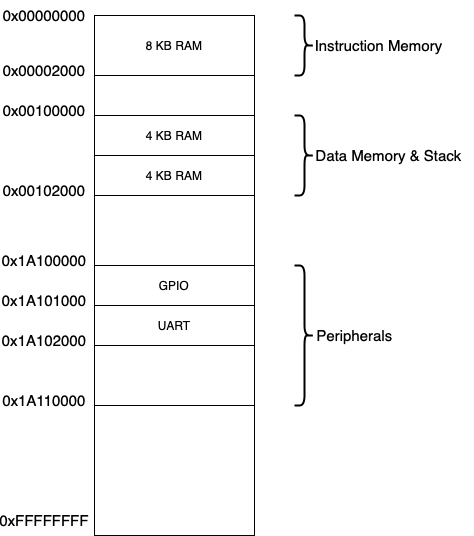
\includegraphics[scale=0.7]{./images/memory}
\caption{MC2101 Memory Map.}
\label{fig:memory} % \ref{fig:memory}
\end{figure}

Figure \ref{fig:memory} shows the default memory map of MC2101. By carefully observing the size of the memory sections it is possible to note that the physical portion of memory currently mapped is in the order of KB, there is a huge free space that can be used in future expansions. In particular the main memory has a lot of available space for being extended to support more advanced software implementations, e.g., hosting an operating system.

The following Subsections are presenting all the possible high-level functions that a programmer can use to write programs for MC2101, maintaining a certain degree of abstraction from the hardware. For this purpose, the GPIO and UART peripherals libraries include a wide amount of functions that, together with macro definitions, allow to program all the functionalities without the need of manually access the user registers manually.

\subsection{GPIO Library}
\begin{table}
\centering
\begin{tabular}{| l | p{7cm} |}
    \hline
    \textbf{Function} & \textbf{Description}\\ \hline
    \texttt{set\_pin\_direction()} & Used to set a pin direction to input or output. \\ \hline
    \texttt{get\_pin\_direction()} & Returns the direction of a given pin. \\ \hline
    \texttt{set\_pin\_value()} & Used to set a pin voltage level to low/high.  \\ \hline
    \texttt{get\_pin\_value()} & Returns a given pin's voltage level.   \\ \hline
    \texttt{set\_pin\_irq\_enable()} & Enable or disable interrupt on a pin.  \\ \hline
    \texttt{get\_pin\_irq\_enable()} & Get the programmed pin's interrupt enable flag.  \\ \hline
    \texttt{set\_pin\_irq\_type()}  & Used to configure the interrupt triggering behavior for a given pin. \{Logic Levels or Edges\}. Pin must have its interrupt flag enabled. \\ \hline
    \texttt{get\_pin\_irq\_type()} & Returns the programmed pin's interrupt triggering behavior.  \\ \hline
    \texttt{get\_gpio\_irq\_status()} & Returns GPIO's current interrupt status register (\texttt{INTSTATUS)} value. Responsible also to deassert the GPIO pending interrupt.  \\ \hline
    \texttt{ISR\_GPIO()} & GPIO interrupt handler. When the interrupt is raised, the bootloader will jump to this function.  \\ \hline
    \hline
\end{tabular}
\caption{GPIO Library functions.}
\label{tab:gpiofunc} % \ref{tab:gpiofunc}
\end{table}

The Table \ref{tab:gpiofunc} shows a simplified prototype and explanation of the GPIO functions currently implemented in the library. The library implements all the necessary functions to be used for programming the peripheral without the need to directly access its registers, thus providing an adequate level of abstraction. The library offers the possibility to configure the direction of each of the 32 pins, read and write values on them. But also, provide a set of functions to be used to enable interrupts on any pin and write a custom interrupt service routine.

\subsection{UART Library}
\begin{table}
\centering
\begin{tabular}{| p{4cm} | p{7cm} |}
    \hline
    \textbf{Function} & \textbf{Description}\\ \hline
    uart\_set\_cfg() &  Used to program the LCR register for configuring the character width, number of stop bits, parity type and enable, even/odd parity and the baudrate.  \\ \hline
    uart\_get\_cfg() &  Return the current LCR register value.\\ \hline
    uart\_set\_int\_en() &  Configure the IER register to enable the different type of interrupt sources. \\ \hline
    uart\_get\_int\_en() &  Used to get the enabled interrupt sources by reading the IER content.\\ \hline
    uart\_rx\_rst() &  Clear the content of the receiver's FIFO.\\ \hline
    uart\_tx\_rst() &  Clear the content of the transmitter's FIFO.\\ \hline
    uart\_set\_trigger\_lv() & Set the receiver's FIFO trigger level.  \\ \hline
    uart\_get\_lsr() &  Used to read the Line Status Register (LSR). \\ \hline
    uart\_get\_isr() &  Used to read the Interrupt Status Register (ISR). \\ \hline
    uart\_sendchar() & Send a character on the transmitter line. \\ \hline
    uart\_getchar() &   Get the character received. \\ \hline
    uart\_send() &  Used to send a string on the transmitter line.\\ \hline
    ISR\_UART() &  UART interrupt handler. When the interrupt is raised, the bootloader will jump to this function. \\ \hline
    \hline
\end{tabular}
\caption{UART Library functions.}
\label{tab:uartfunc} % \ref{tab:uartfunc}
\end{table}

The UART library offers a bigger set of functions with respect to the GPIO library, functions that are also more complex (in terms of execution time) because also the UART features are more complicated. The library provides the possibility to configure the speed of the communications, the size of the frames transmitted/received as well as all the error detection mechanisms. Provides to the programmer functions able to send single characters or strings, and to customise the interrupt behavior.\\
More details about the library are reported in Table \ref{tab:uartfunc}.

\subsection{String Library}
More advanced I/O functionalities have been implemented in the \emph{string} library. This library is particularly important, because it provides the principal string manipulations functions that together with the UART Library are able to support the \texttt{printf} and \texttt{scanf} functions. The library is the same implemented in PULPino, with the addition of the \texttt{scanf} function and some other utilities. The following functions are part of the system's library:
\texttt{strlen}, \texttt{strcpy}, \texttt{strcmp}, \texttt{puts}, \texttt{putchar}, \texttt{memset}, \texttt{printf} and finally the \texttt{scanf}.

\subsection{Board Library}
This is the ``top-level'' library that should be included in every application developed for MC2101. It contains the \texttt{board\_setup} function, which was prepared right after the pin planning phase. It is used to initialize the microcontroller hardware once synthesized on FPGA and connected with the various user buttons, switches and LEDs present in the board.

Once called, the microcontroller is configured in this way:
\begin{itemize}
\item UART peripheral is programmed with 115200 standard baudrate, no parity, 1 stop bit, 8-bit character width. This is a standard configuration for the \texttt{printf} and \texttt{scanf} functions.
\item GPIO lines interconnected to LEDs are set as output.
\item GPIO lines interconnected to User buttons are set as input.
\item GPIO lines interconnected to Switches are set as input.
\item Al interrupts are disabled.
\end{itemize}
The \texttt{board\_setup} function should be the first called in every application, because brings the microcontroller in the correct configuration, according to the pin assignment used for the synthesis, in order to properly interface the external hardware.

\section{Testing}
The microcontroller has been tested with the combination of RTL testbenches and C programs, aimed together to verify the correctness of the architecture. The original AFTAB simulation environment, similar to PULPino, has been adopted and extended for the test of MC2101.

As anticipated, the software environment integrates the RISC-V toolchain with ModelSim commands using CMake build automation tool. In this way, it is possible to compile custom C applications, HDL design files, and also run RTL simulations on ModelSim.

The test of the architecture has been separated into two distinct phases:
\begin{enumerate}
\item Testing while-developing.
\item Testing post-synthesis on FPGA.
\end{enumerate}  

\subsection{Testing while-developing}
Test activities and design activities happened in parallel during the RTL development of the microcontroller. All the components have been implemented using a structural approach in such a way to have a modular design, easily testable with a bottom-up methodology.

\begin{figure}[h]
\vspace{0.5cm}
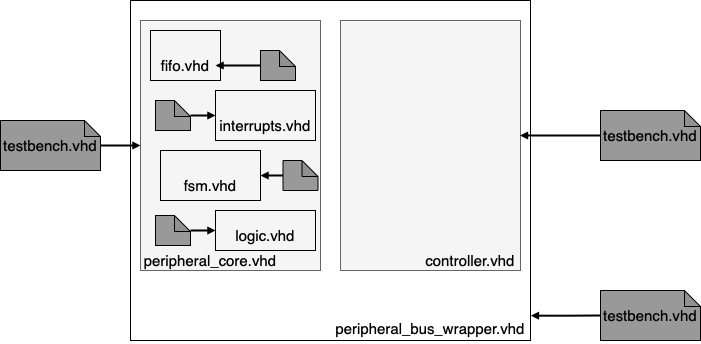
\includegraphics[scale=0.6]{./images/testing}
\caption{Modular structure of a peripheral.}
\label{fig:testing} % \ref{fig:testing}
\end{figure}

Figure \ref{fig:testing} shows what is the typical structure used to design all the peripherals. There is always a top-level entity, that works as a wrapper for the bus controller and the peripheral core, which is itself composed of discrete interconnected HDL entities. Each of the entities is at first tested in isolation, then in integration with the other components until the design is functionally tested from the bottom to the top-level entity. The peripheral can be then attached to the bus, through the top-level wrapper, and be finally tested with a proper C/Assembly program to verify the correctness of the interconnection with the processor and the memory. With this approach, the microcontroller can be testes bottom-up, and debugged with custom applications. After these steps, the final test would be to proceed with the synthesis of the design and perform a last RTL test with a gate-level simulation, to properly check that timing constraints are really respected. 

\subsection{FPGA Tests}
The test procedure explained before is not actually able to fully test all the functionalities because of the limitations of RTL simulations. Interrupts for instance, are ver difficult to test, because they should be generated asynchronously by the external environment, e.g., a button press. Other behaviors like the \texttt{printf} or \texttt{scanf} functions would require very long simulation times (in the order of ms) that can really overload ModelSim, with the risk of crashing the workstation.

In general, the functional properties of the microcontroller can be fully tested only when synthesized on FPGA, that in our case is the Cyclone-V FPGA embedded into the DE1-SoC development board. With the purpose of having a proper test infrastructure, a set of make targets, integrating Quartus commands with tcl and bash scripts have been prepared in order to provide to the user a simple, fast and automatic toolchain for the synthesis and deployment on FPGA. The most useful feature of the aforementioned toolchain, is certainly the possibility of updating the memory content of the sythesized microcontroller with new programs, without having to repeat the entire synthesis process from scratch, which can be quite time consuming.

Below, are presented some more details about the testing of the UART and GPIO peripherals, thus are also showed the different ways of interacting with the microcontroller.

\begin{figure}[h]
\centering
\vspace{0.5cm}
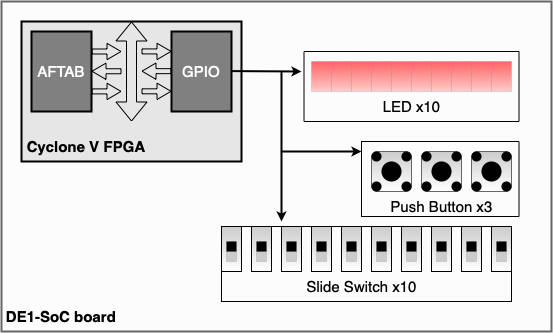
\includegraphics[scale=0.6]{./images/gpiotesting}
\caption{GPIO Interconnection on DE1-SoC.}
\label{fig:gpiotesting} % \ref{fig:gpiotesting}
\end{figure}

\textbf{The GPIO peripheral} is interconnected with a proper set of component present on the DE1-SoC. As shown in Figure \ref{fig:gpiotesting}, there are 10 LEDs in total, 3 push buttons, and 10 switches that are physically connected with the GPIO's External Interface lines. This set of electronic components are very useful in order to test the behavior of the peripheral, the user can assess if the peripheral works or not by just trying to turn on/off LEDs. Test programs have been implemented with the purpose to check the functional correctness of the the whole peripheral and the interrupt mechanism.

\textbf{The UART peripheral} has been tested together with the \texttt{printf} and \texttt{scanf} functions. In this case, the test is a little bit more complicated, as it requires the usage of a Terminal Emulator in order to see if the I/O functions are working. 

\begin{figure}[h]
\vspace{0.5cm}
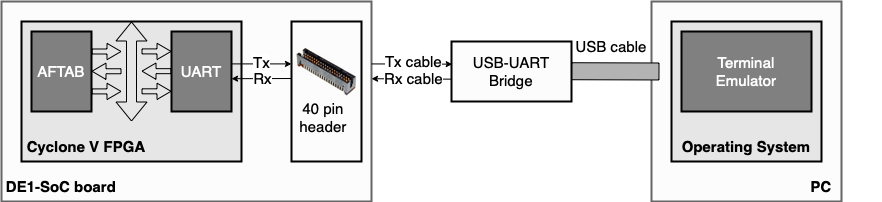
\includegraphics[scale=0.5]{./images/uarttesting}
\caption{UART Interconnections.}
\label{fig:uarttesting} % \ref{fig:uarttesting}
\end{figure}

In Figure \ref{fig:uarttesting}, the communication mechanism designed for interconnecting the UART peripheral with an external PC is shown. The interconnection is very simple, the \texttt{tx} and \texttt{rx} lines have been routed with 2 header pins of the DE1-SoC, then two cables are used to connect the \texttt{tx} and \texttt{rx} lines to a USB-UART bridge that is directly plugged into USB Port of a computer. In this way, every Terminal Emulator is able to print the character transmitted by the microcontroller and also send character to the microcontroller. This communication mechanism, together with the GPIO connections allow a proper test of the entire microcontroller.